\documentclass[12pt]{article}
\usepackage[english]{babel}
\usepackage{lipsum}
\usepackage[square, numbers]{natbib}
\bibliographystyle{plainurl}
\usepackage{url}
\usepackage[utf8x]{inputenc}
\usepackage{amsmath}
\usepackage{mathtools,siunitx}
\sisetup{detect-all}
\usepackage{graphicx}
\graphicspath{{images/}}
\usepackage{parskip}
\usepackage{fancyhdr}
\usepackage{vmargin}
\usepackage{hyperref}
\usepackage{todonotes}
\usepackage{textcomp}
\usepackage{float}
\usepackage{listings}
\usepackage{enumitem}
\usepackage{caption}
\usepackage{listings}


\usepackage{color} %red, green, blue, yellow, cyan, magenta, black, white
\definecolor{mygreen}{RGB}{28,172,0} % color values Red, Green, Blue
\definecolor{mylilas}{RGB}{170,55,241}
\setmarginsrb{2 cm}{2.5 cm}{2 cm}{2.5 cm}{1 cm}{1 cm}{1 cm}{1 cm}
\presetkeys{todonotes}{fancyline}{}

%%%%%%%%%%%%%%%%%%%%%%%%%% TITLE %%%%%%%%%%%%%%%%%%%
\title{Pulse Modulation Techniques and Observations of the Atmosphere}
\author{A. Scharf}	
\date{\today}

\makeatletter
\let\thetitle\@title
\let\theauthor\@author
\let\thedate\@date

\providecommand\add@text{}
\newcommand\tagaddtext[1]{%
  \gdef\add@text{#1\gdef\add@text{}}}% 
\renewcommand\tagform@[1]{%
  \maketag@@@{\llap{\add@text\quad}(\ignorespaces#1\unskip\@@italiccorr)}%
}
\makeatother

\pagestyle{fancy}
\fancyhf{}
\rhead{\theauthor}
\lhead{\thetitle}
\cfoot{\thepage}

\renewcommand{\thesubsection}{\thesection.\alph{subsection}}



\begin{document}

\lstset{language=Matlab,%
    %basicstyle=\color{red},
    breaklines=true,%
    morekeywords={matlab2tikz},
    keywordstyle=\color{blue},%
    morekeywords=[2]{1}, keywordstyle=[2]{\color{black}},
    identifierstyle=\color{black},%
    stringstyle=\color{mylilas},
    commentstyle=\color{mygreen},%
    showstringspaces=false,%without this there will be a symbol in the places where there is a space
    numbers=left,%
    numberstyle={\tiny \color{black}},% size of the numbers
    numbersep=9pt, % this defines how far the numbers are from the text
    emph=[1]{for,end,break},emphstyle=[1]\color{red}, %some words to emphasise
    %emph=[2]{word1,word2}, emphstyle=[2]{style},
}

%%%%%%%%%%%%%%%%%%%% Titlepage start %%%%%%%%%%%%%%%%%%%%%%%%%%%%

\begin{titlepage}
	\centering
    \vspace*{0.5 cm}
    
\includegraphics[scale = 0.4]{images/lulea}\\[1.0 cm]

   	\vspace{2cm}
	\textsc{\Large Optics- and Radar-based Observations}\\[0.5 cm]

	\textsc{\large F7003R}\\[0.5 cm]	
	\rule{\linewidth}{0.2 mm} \\[0.4 cm]
	{ \huge \bfseries \thetitle}\\
	\rule{\linewidth}{0.2 mm}
	\\[0.5cm]
		\textsc{}
		\\[2.5 cm]

	
	\emph{Author:}\\
	Arthur Scharf
	\vspace{2cm}
	
	{\large \today }\\[2 cm]
 
	\vfill
	
\end{titlepage}
%%%%%%%%%%%%%%%%%%% Titlepage end %%%%%%%%%%%%%%%%%%%%%%%%%%%%%%%


%%%%%%%%%%%%%%%%% include content %%%%%%%%%%%%%

%%%%%%%%%%%%%%%%% Introduction to the Assignment %%%

In this Assignment, \textit{\textbf{Problem 2 - general radar theory}}, ...


%%%%%%%%%%%%%%%%% TASK 1 %%%
\section{Operational frequency for scientific radar}
The operational frequency for a scientific radar is highly depending on the application and the type of the target. If for example the ionosphere, a so-called soft-target is to be observed, the range resolution of the radar plays a more important role than for example when a hard target is wanted. 


\subsection{Frequency ranges}
Radar stands for \textit{\textbf{Radio Detection and Ranging}}, so Radar generally operates in the RF band, going from about 3MHz to 300GHz \citep{richards2010principles}. Therefore, any of the Radar techniques explained above can be operated in any of those ranges. However, some specific frequency ranges may have advantages and disadvantages for the particular radar technique applied, which is why sometimes ISR, CSR and Doppler Radar Applications are categorized in different bands. Unfortunately, different literature and papers state different ranges. For example the University of Oslo states, ISR ranges from between 50MHz up to 2 GHz, \citep{oslo:lecture}, whereas Tromso for example uses UHF and VHF radar with frequencies between 224 and 933 MHz. For CSR usually a range between 3 and 300MHz is used.

Doppler radar though can be used in almost every RF range, also called bands (c.f. \ref{tab:bands}).

\begin{table}[h!]
\centering
\caption{Different frequency bands used in radar}
\label{tab:bands}
\begin{tabular}{|c|c|l|}
\hline
\textbf{Band name} & \textbf{Frequency} & \textbf{Usage}                    \\ \hline
HF                 & 3-30 MHz           & Coastal radar systems             \\ \hline
L                  & 1-2 GHz            & Long range air traffic control    \\ \hline
S                  & 2-4 GHz            & weather, marine radar             \\ \hline
C                  & 4-8 GHz            & satellite transponders, weather   \\ \hline
X                  & 8-12 GHz           & weather, mapping, military        \\ \hline
K                  & 18-24 GHz          & limited usage (water vapour)      \\ \hline
V                  & 40-75 GHz          & limited (oxygen absorption)       \\ \hline
W                  & 75-110 GHz         & high-res mapping and observations \\ \hline
\end{tabular}
\end{table}


\subsection{Information gathered by radar measurement}

The incoherent scatter radar is mostly used for ionospheric research and observations. The ISR radar beam scatters off of electrons in the ionospheric plasma, which then can be captured by an appropriate radar. The fluctuation in electron density provides information about the ion temperature, mass distribution as well as ion composition and plasma velocity (using Doppler radar, in this case) \citep{gordon1958incoherent}.

The working principle Coherent Scatter Radar is similar to the ISR, it also relies on backscattering off of plasma waves and thus can observe them. Combining multiple radars allows to track plasma flows on a very large scale. But since no direct plasma parameters are measured (as in case of ISR), one must be cautious in interpreting data. 

Doppler radar is different in its working principle. Doppler relies on the fact that an electromagnetic wave needs some time to propagate to its destination. Since the propagation speed of the wave is known, one can determine the distance of where the EM wave was reflected with the help of very precise measurement of the reflected wave. Also, the velocity of the observed target can be determined.



%%%%%%%%%%%%%%%%% TASK 2 %%%
\section{The radar equation}
To derive the radar equation one starts with the assumption of an isotropic radiation source. Therefore the power density at a distance R is denoted as


\begin{equation}
\label{eq:iso}
	\centering
	Q_{i} = \frac{P_t}{4 \pi R^2} \qquad \bigg[\frac{W}{m^2} \bigg]
\end{equation}

Since usually radar is focused in one specific direction, the equation is multiplied with the Gain G of the antenna

\begin{equation}
\label{eq:dir}
	\centering
	Q_{i} = \frac{P_t G}{4 \pi R^2} \qquad \bigg[\frac{W}{m^2} \bigg]
\end{equation}

When the radiated power now hits a target, a fraction of the power is reflected, or \textit{re-radiated}. This reradiated power is depending on the cross-section $\sigma$ of the hit target. So the received Power density at the antenna is 

\begin{equation}
\label{eq:rePowDen}
	\centering
	Q_{re} = \frac{Q_i \sigma}{4\pi R^2} = \frac{P_t G}{4 \pi R^2} \frac{\sigma}{4\pi R^2} \qquad \bigg[\frac{W}{m^2} \bigg]
\end{equation}

But this received Power is now again dependent on the antenna gain, which is in this case also depending on the antenna effective area $A_{eff}$

\begin{equation}
\label{eq:rePow}
	\centering
	P_{r} = Q_{re} A_{eff} = \frac{P_t G}{4 \pi R^2} \frac{\sigma}{4\pi R^2} A_{eff}\qquad [W]
\end{equation}

The antenna effective area can now be expressed with the help of the antenna gain. The derivation of the gain is not shown here, but it can be derived using the effective area of a Hertzian dipole and the assumption that the antenna perfectly absorbs all received power.\par
This leads to the equation for the antenna effective area, which is depending on the antenna gain and the wavelength $\lambda $ of the used frequency.

\begin{equation}
\label{eq:Aeff}
	\centering
	A_{eff} = G \frac{\lambda^2}{4\pi} \qquad [m^2]
\end{equation}

Inserting this relation in equation \ref{eq:rePow} leads to the so-called Radar Equation, the total received power of the antenna.

\begin{equation}
\label{eq:radEq}
	\centering
	P_{r} = P_t \frac{\rho_a^2 A^2 }{4 \pi \lambda^2 R^2} \sigma \qquad [W]
\end{equation}

where $\rho_{a} $ is the antenna efficiency, defined as

\begin{equation}
\label{eq:effi}
	\centering
	\rho_a = \frac{\lambda^2 G }{4 \pi A} = \frac{A_{eff}}{A}
\end{equation}

with $A$ being the total antenna area.

This derivation was done keeping in mind that only one target, a so-called hard target is being observed. In case of a distributed, or soft target the equation \ref{eq:radEq} is further enhanced.

To generalize the equation \ref{eq:radEq} for more than one target over a volume, one can use the integral relation of cross sectino areas in a Volume (\ref{eq:crossVol}).

\begin{equation}
	\label{eq:crossVol}
	\centering
	\int \sigma(\vec{x}) dV_s \equiv \sigma
\end{equation}

Inserting this into Eq. \ref{eq:radEq} leads to a generalized version Equation.

\begin{equation}
\label{eq:radEqGen}
	\centering
	P_{r} = \int P_t \frac{\rho_a^2 A^2 }{4 \pi \lambda^2 R^2} \sigma(\vec{x}) dV_s \qquad [W]
\end{equation}


\begin{figure}
	\centering
	\label{fig:softTarget}
	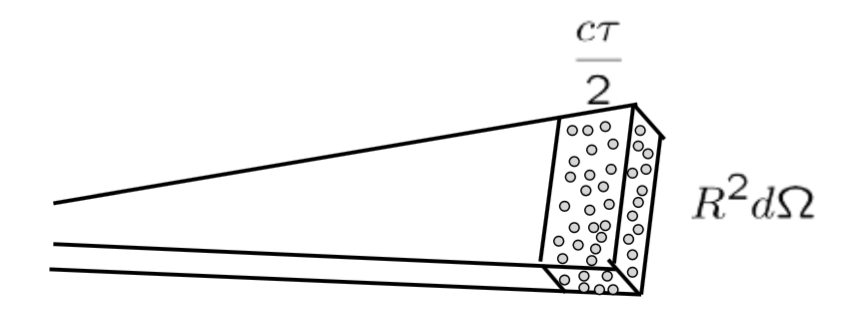
\includegraphics[width=0.8\textwidth]{images/softTarget}
	\caption{Soft Target (image source: lecture by Philip Erickson \citep{erickson:lecture})}
\end{figure}

Assuming an isotropic scatter distribution for the volume (c.f. \ref{fig:softTarget}), one can solve the integral to:

\begin{equation}
	\label{eq:crossVol}
	\centering
	\int \sigma(\vec{x}) dV_s = \frac{ c \tau}{2} R^2 \sigma
\end{equation}

Combining (\ref{eq:crossVol}) and the generalized radar equation (\ref{eq:radEqGen}) leads to the radar equation for a soft target:

\begin{equation}
\label{eq:radEqSoft}
	\centering
	P_{r} = P_t \frac{c \rho_a^2 A^2 \tau}{8 \pi \lambda^2 R^2} \sigma \qquad [W]
\end{equation}


%%%%%%%%%%%%%%%%% TASK 3 %%%
\section{Cross section calculation}
To calculate the minimum cross section that is detectable for the given values

\begin{center}
\begin{tabular}{c c}
	Object Location & $R$ = 100km \\
	Wavelength & $\lambda$ = 6m \\
	Transmit Power & $P_t$ = 10 kW \\
	Antenna Gain & $G$ = 20 dB = 100 W\\
	System Noise Temperature & $T_s$ = $10^3$ K \\
	Bandwith & $B_w$ = 1 MHz
\end{tabular}
\end{center}

the Signal-to-Noise ratio (SNR) is used. The SNR is the ratio between the received power versus the total system noise Power, where the System Noise Power is, according to \todo{richards zitieren}, denoted as

\begin{equation}
\label{eq:noise}
	\centering
	P_n = N_0 = k_B T_s B_w \qquad [W]
\end{equation}

Using equations \ref{eq:rePow} and \ref{eq:noise}, the SNR can be written as

\begin{equation}
\label{eq:snr}
	\centering
	SNR = \frac{P_r}{P_n} = \frac{P_t G A_{eff} \sigma}{4 \pi R^2 k_B T_s B_w}
\end{equation}

Substituting $A_{eff}$ with eq. \ref{eq:Aeff} and re-ordering \ref{eq:snr} to the cross section area $\sigma$ leads to

\begin{equation}
\label{eq:snr}
	\centering
	\sigma = {SNR} \frac{(4 \pi)^3 R^4 k_B T_s B_w}{P_t G^2 \lambda^2}	\qquad [m^2]
\end{equation}

To calculate the smallest cross section area that is detectable at a range of 100km, one has to assume a minimum SNR, at which the minimum cross section is still detectable.

The minimum SNR, not taking into account LNA's or other instruments to increase the SNR, is obviously 1, since if the signal is stronger than the noise the signal is theoretically detectable.

Inserting $SNR_{min} = 1$ for SNR in eq. \ref{eq:snr} this leads to a minimum cross section

\begin{equation}
\label{eq:crossSecResult}
	\centering
	\sigma_{min} = 0.76105 \qquad [m^2]	
\end{equation}

This is the same result as is given in the assignment sheet.


%%%%%%%%%%%%%%%%% TASK 4 %%%
\section{MST radars}

\subsection{SNR as function of universal time and altitude}
To plot the Signal to Noise ratio as a function of time and altitude, data from 28th of February 2006 is used. The plot can be seen in fig. \ref{img:snrPlot}, the MATLAB Code used to plot these heatmaps can be found in Appendix \ref{code:snr}.

\begin{figure}
	\centering
	\label{img:snrPlot}
	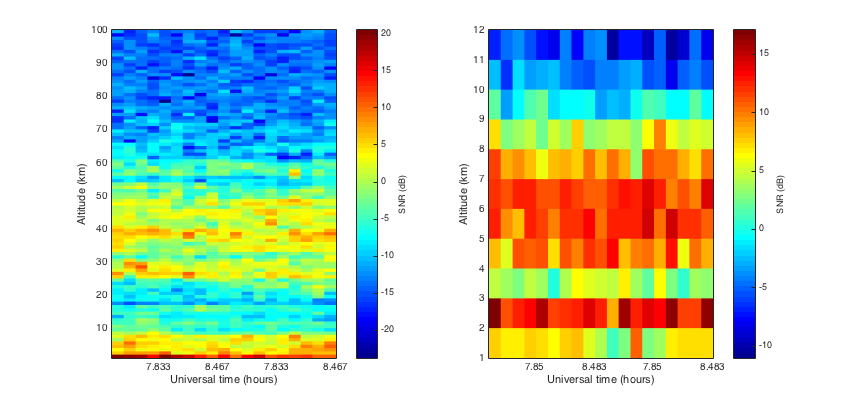
\includegraphics[width=\textwidth]{images/task4_plot1}
	\caption{SNR as function of altitude and time, data from 28Feb06}
\end{figure}


\subsection{Pulse calculations}
To calculate the pulse length, the inter-pulse period (IPP), pulse repetition frequency (PRF )and maximum unambiguous range 	$R_{max}$ for these height resolutions, the following formulas are used:

\begin{center}
\begin{equation}
\centering
\label{eq:pulselength}
	\Delta R = \frac{c \tau_p }{2} \qquad [km] \qquad \textrm{, with } \Delta R \textrm{ as Range resolution and } \tau_p \textrm{ as pulse length}
\end{equation}
\begin{equation}
\label{eq:ipp}
	{IPP} = \frac{\tau_p }{D} \qquad [s] \qquad \textrm{, with D as duty cycle}
\end{equation}
\begin{equation}
\label{eq:prf}
	PRF = \frac{1}{IPP} \qquad [Hz]
\end{equation}
\begin{equation}
\label{eq:rangeMax}
	R_{max} = \frac{c \,  {IPP} }{2} \qquad [km]
\end{equation}
\end{center}

Using these equations the appropriate values for each height resolution is calculated. For the Duty Cycle a value of 5\% is assumed.

\begin{center}
\begin{table}
\label{tab:range}
	\caption{Calculated values using eq. (\ref{eq:pulselength}) to (\ref{eq:rangeMax})}
\begin{center}
\begin{tabular}{ |c | c | c|}
	\hline
	\textbf{Range resolution} & \textbf{150m} & \textbf{1200m} \\
	\hline
	\textbf{Pulse Length} & 1 $\mu s$ & 8 $\mu s$ \\
	\textbf{IPP} & 20 $\mu s$  & 160 $\mu s$ \\
	\textbf{PRF} & 50 kHz & 6250 Hz\\
	\textbf{ R$_{max}$} & 3 km & 24 km\\
	\hline	
\end{tabular}
\end{center}
\end{table}
\end{center}


\subsection{Transmitted pulse length and received signal strength}

Using equations \ref{eq:ipp} and \ref{eq:prf} as well as the relation of Peak to average power (\ref{eq:avg}) one can combine those and get the transmitted Power in relation of to the transmitted pulse length $\tau_p$ (c.f. eq. \ref{eq:transmittedPower}).

\begin{equation}
	\centering
	\label{eq:avg}
	P_{avg} = P_t D = (\tau_p \textrm{PRF} )
\end{equation}

\begin{equation}
	\centering
	\label{eq:transmittedPower}
	P_{t} = \frac{P_{avg} T_d}{\tau_p n_p} 
\end{equation}

With $n_p$ being the number of pulses, in this case one, and the dwell-time 
\begin{equation}
	\label{eq:dwell}
	\centering
	T_d = \frac{n_p}{\textrm{PRF}}
\end{equation}

the transmitted power $P_t$ can be substituted in eq. \ref{eq:radEq}, which leads to the total received power related to the transmitted pulse length (\citep[c.f.][chap. 2.10]{richards2010principles}):


\begin{equation}
	\label{eq:relation}
	\centering
	P_r = \frac{P_{avg} T_d \rho^2 A^2 \sigma }{\tau_p 4 \pi \lambda^2 R^2} \qquad	[W]
\end{equation}

\subsection{Atmospheric parameters}

The radar observes the atmosphere up to a height of about 17 km, thus the radar is observing the troposphere (0 to 12km) and lower parts of the stratosphere (12 to 50km).

One can observe that up to height of about 3km the SNR is quite high, presumably this is the case of the dense atmosphere near ground, for example clouds or fog. Between 3 and 6 the SNR gets lower, with then having a region with higher SNR up to about 11km.

It seems that the wind is causing this increase in SNR, since plotting the wind data provided in addition to the SNR and altitude data (when available) reveals that the wind in these attitude is quite strong, with absolute wind speeds up to 10 m/s




% if appendix needed, uncomment the following lines
%\section*{Appendix}
%%\addtocontents{toc}{\protect\setcounter{tocdepth}{1}}
%\renewcommand{\thesection}{\Alph{subsection}}
%\setcounter{section}{1}
\renewcommand{\thesubsection}{\thesection.\arabic{subsection}}
\appendix
\section{Appendix}

\subsection{MATLAB Code for Tasks 1 to 8 }
\label{apdx:matlab}
\begin{center}
	\lstinputlisting[language=Matlab,caption={Matlabcode for antenna design calculations and plots}]{appendix/phasedArray.m}
\end{center}


% if bibliography needed, uncomment the following lines
\bibliographystyle{plainnat}
\bibliography{biblist}

%%%%%%%%%%%%%%%%% include content end %%%%%%%%%
\end{document}
